\documentclass[a4paper,DIV=12,english]{scrartcl}
\usepackage[utf8]{inputenc}
\usepackage{graphicx}
\usepackage{hyperref}
\usepackage{csquotes}
\usepackage{amsthm}
\usepackage{amssymb}
\usepackage{bbm}
\usepackage{amsmath}
\usepackage{tikz}
\usepackage{svg}
\usepackage{braket}
\usepackage{caption}
\usepackage{subcaption}
\usepackage{placeins}
% Fakesection
\newcommand{\fakesection}[1]{%
    \par\refstepcounter{section}                                        % Increase section counter
    \sectionmark{#1}                                                    % Add section mark (header)
    \addcontentsline{toc}{section}{\protect\numberline{\thesection}#1}  % Add section to ToC
    % Add more content here, if needed.
} 

\renewcommand{\thesubsection}{\thesection.\alph{subsection}}

\title{Data and Signal Analysis\\Problem Sheet 1}
\author{Elise Pilgermann, Max Maschke}
\date{\today}

\begin{document}
\maketitle
\setcounter{section}{1}
\section{Analysing a time series}

\subsection{}
\begin{figure}
    \centering
    \begin{subfigure}{0.49\textwidth}
        \centering
        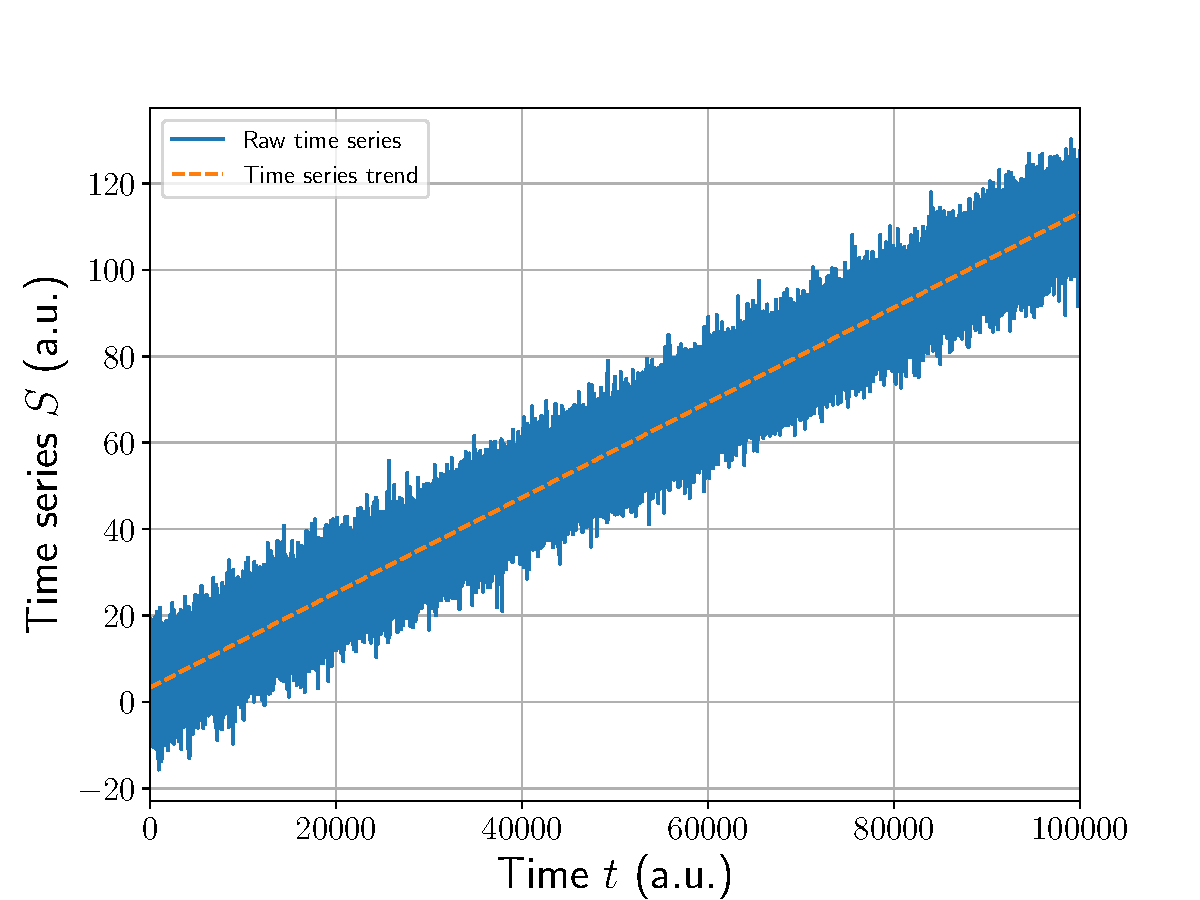
\includegraphics[width=\textwidth]{../timeseries_trend_plot.pdf}
        \caption{}
        \label{fig:ts_trend}
    \end{subfigure}
    \begin{subfigure}{0.49\textwidth}
        \centering
        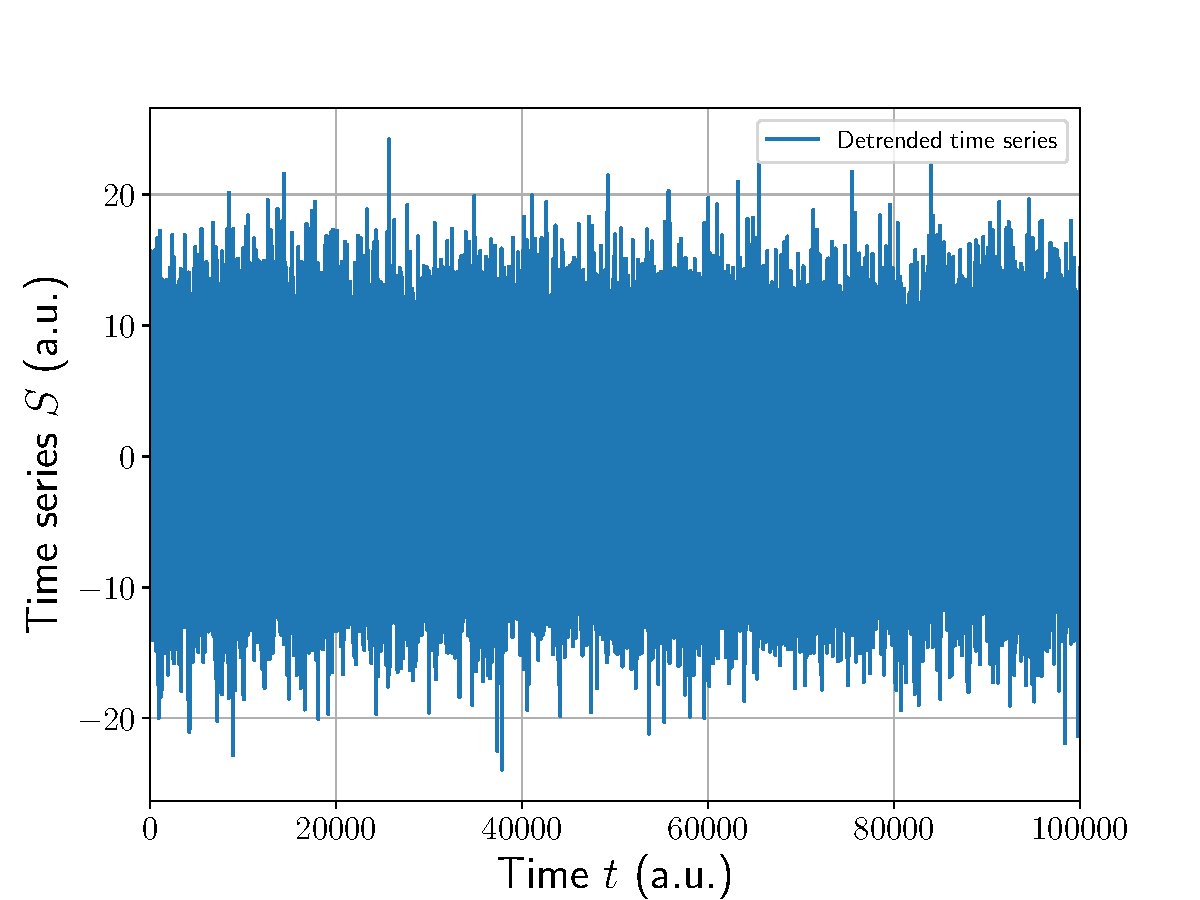
\includegraphics[width=\textwidth]{../timeseries_detrended.pdf}
        \caption{}
        \label{fig:ts_detrended}
    \end{subfigure}    
    \caption{Time series given in \texttt{timeseries.txt} including trend obtained through linear regression \ref{fig:ts_trend} and detrended using said fit \ref{fig:ts_detrended}.}
    \label{fig:ts}
\end{figure}
The time series is shown in figure~\ref{fig:ts_trend}. We notice a trend in the data that is clearly linear over the given interval.

\subsection{}
To detrend the time series, we perform a linear regression, i.e.\ a least squares fit to a function $S(t)=\alpha t + \beta $, using the \texttt{linregress} function from the \texttt{scipy.stats} module. We obtain the parameters
\begin{equation*}
    \alpha = 0.00109956 \pm 5.8\cdot 10^{-7}, \quad \beta = 3.318 \pm 0.034
\end{equation*}
and an $R^2$-value of $0.986$. The fit is also shown as the dashed line in figure~\ref{fig:ts_trend}, and it can clearly be seen that it approximates the underlying trend well.

To detrend the time series, we simply subtract the value of the fitted trend function from the data at every discrete time step. This results in a noisy modified series shown in figure~\ref{fig:ts_detrended}.

\subsection{}
\begin{figure}
    \centering
    \begin{subfigure}{0.49\textwidth}
        \centering
        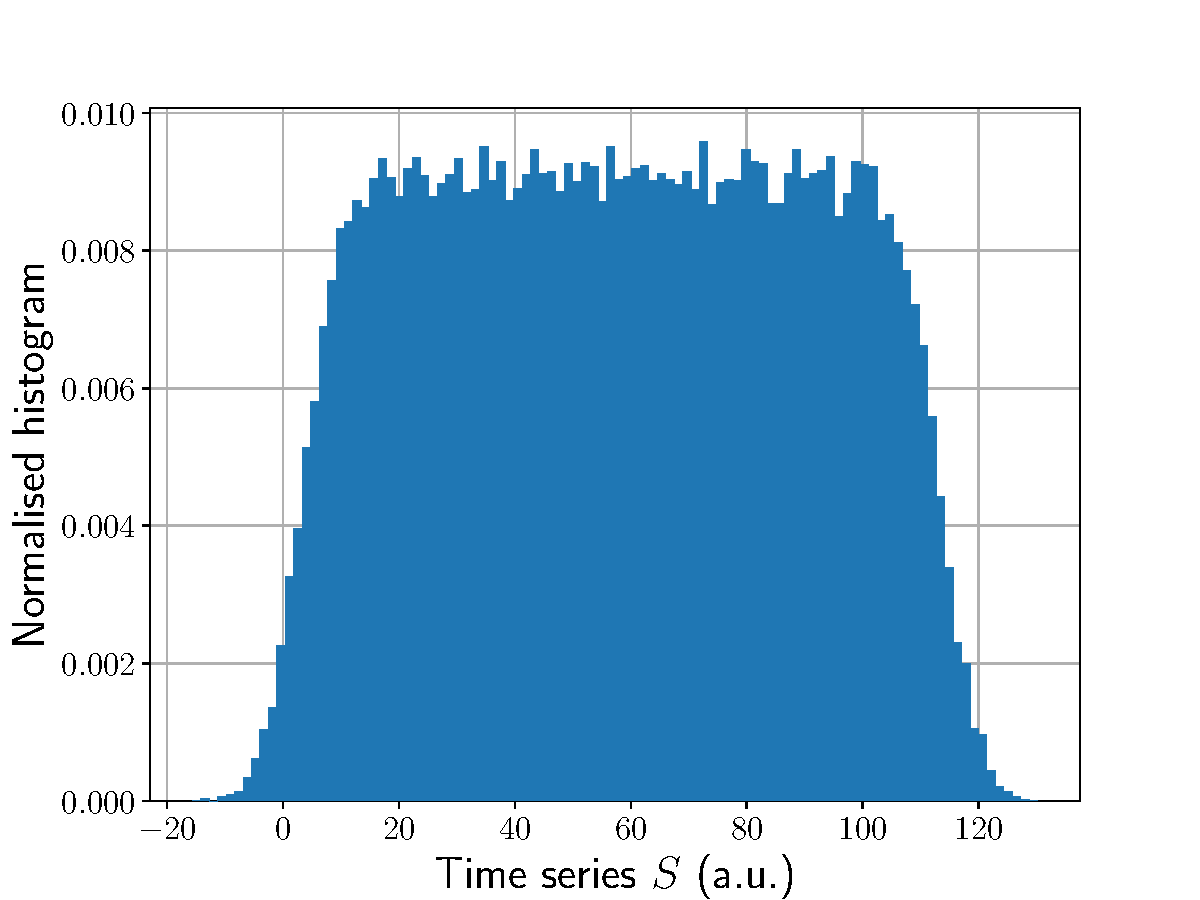
\includegraphics[width=\textwidth]{../timeseries_hist.pdf}
        \caption{}
        \label{hist}
    \end{subfigure}
    \begin{subfigure}{0.49\textwidth}
        \centering
        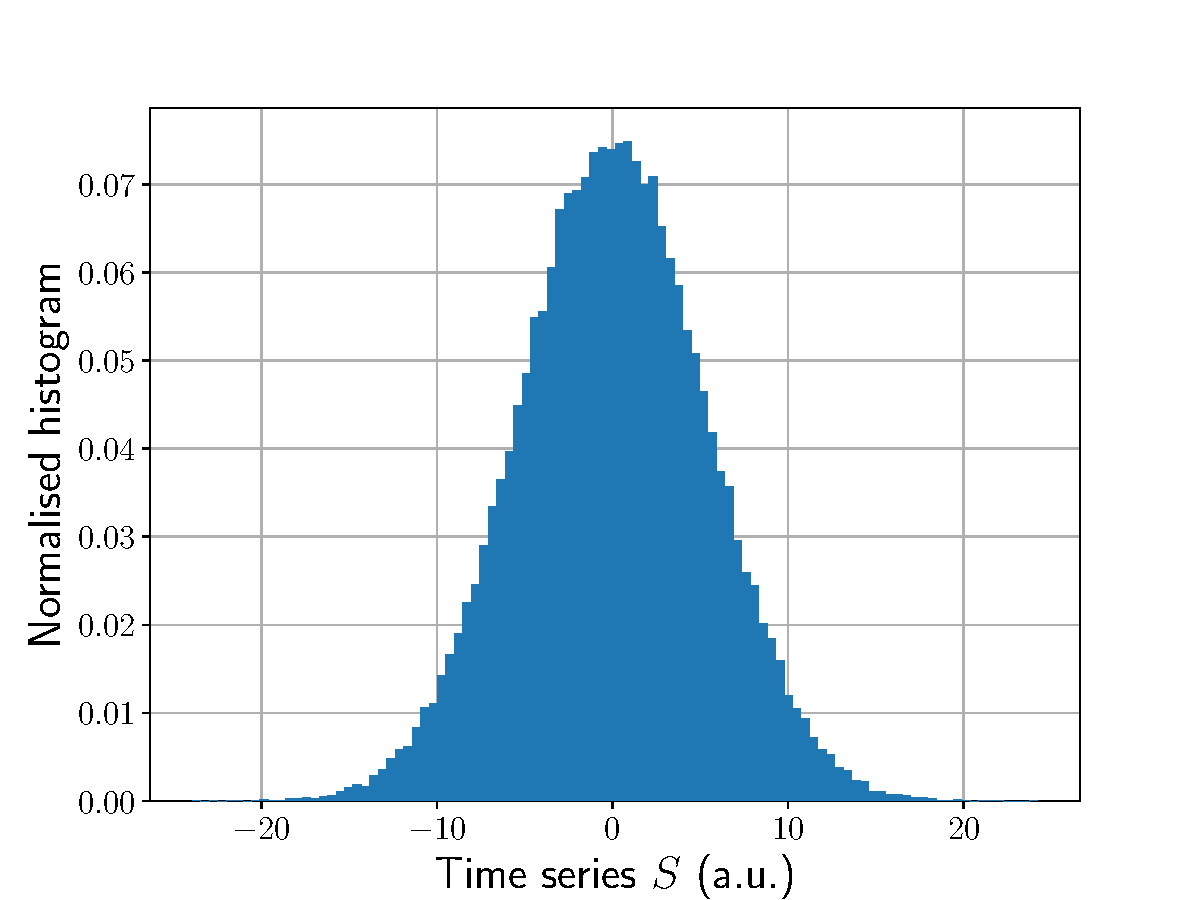
\includegraphics[width=\textwidth]{../timeseries_hist_detrended.pdf}
        \caption{}
        \label{hist_detrended}
    \end{subfigure}
    \caption{Histogram of the raw time series \ref{hist} and of the detrended time series \ref{hist_detrended}.}
    \label{fig:hists}
\end{figure}
The raw and detrended histograms are shown in figure~\ref{fig:hists}. The histogram of the raw time series in figure~\ref{hist} is very flat over most of the span of the $x$-range, dropping of quickly at its edges. Assuming a symmetric distribution in the deviation from the linear trend, all values that the trend function assumes should be approximately equally likely to appear in the time series, so the raw histogram should approximately look like a uniform distribution except for the edges where the distribution of the deviation from the trend \enquote{shines through}.

The suspicion that the deviation follows an approximately symmetric distribution is confirmed by inspecting the detrended histogram, \ref{hist_detrended}. It has an approximately Gaussian shape (this is not just the flawed judgement of the eye but will be underpinned by later analysis) with a slight skew to the right of the origin.

In the limit of $\alpha\longrightarrow 0$, both histograms will be identical. Conversely, in the limit of $\alpha\longrightarrow\infty$, the distribution of the raw time series will become even broader and tend to zero (while staying normalised). As long as a good fit of the trend is still possible, the histogram of the deviation should not change noticably.

\subsection{}
Normalised empirical histograms for datasets can be conveniently obtained using the \texttt{histogram} function from the \texttt{numpy} module (care must be taken to call it with the optional parameter \texttt{density=True}).

The histogram is returned as a vector containing the values of the histogram in the bins, so the empirical centered moments can be conveniently calculated as
\begin{equation}
    m_n = \text{d}x \cdot (x - \mu)^n \cdot h
\end{equation}
where $h$ is the histogram vector, $x$ is a linearly spaced vector spanning the range of the dataset, $\mu$ is the mean of the dataset and $\text{d}x$ is the separation of the bins.

The moments obtained in this way are shown in table~\ref{tab:moments}. The 0-th order moments are equal to unity as expected. The first order moment is approximately equal to zero for both histograms because they are centered, otherwise they should yield the mean. The second order moments give the variance. The third order moment is the skewness of the histogram, which is small for both but especially that of the deviation, i.e.\ the detrended time series. The positive sign indicates that both show a small skew to the right of the mean. The fourth order moment, the kurtosis, divided by the variance squared is exactly equal to three for a Gauussian. In our case, we get a value of 3.011, showing that it is very close to a Gaussian and was likely sampled from one.
\begin{table}
    \centering
    \caption{Empirical centered moments of the histograms of the raw and detrended time series.}
    \begin{tabular}{c||c|c}
        Order & Raw time series & Detrended time series \\ \hline
        0 & 1 & 1\\
        1 & 0.00118 & -8.8$\cdot 10^{-5}$\\
        2 & 1040 & 28.2\\
        3 & 22.0 & 0.645 \\
        4 & 2010000 & 2400 \\        
    \end{tabular}
    \label{tab:moments}
\end{table}

\end{document}